\documentclass[10pt,aspectratio=169,handout]{beamer}

\usepackage[utf8]{inputenc}
\usepackage[ngerman]{babel}
\usepackage{utopia}
\usetheme{Darmstadt}
\usecolortheme{default}
\usepackage{xcolor}
\usepackage{graphicx}
\usepackage{amsmath}
\usepackage{amsthm}
\usepackage{amssymb}
\usepackage{amsfonts}
\usepackage{mathtools}
\usepackage{dsfont}
\usepackage{hyperref}
\usepackage[most]{tcolorbox}
\usepackage{tikz}
\usepackage{adjustbox}
\usepackage{mathrsfs}
\usepackage{minted}
\usetikzlibrary{cd}
\usetikzlibrary{positioning}
\usetikzlibrary{calc}
\usetikzlibrary{arrows.meta}
\setbeamertemplate{theorems}[numbered]
\setbeamertemplate{navigation symbols}{}
\newtranslation[to=ngerman]{Theorem}{Satz}
\def\C{\mathbb{C}}
\def\R{\mathbb{R}}
\def\Q{\mathbb{Q}}
\def\N{\mathbb{N}}
\def\Z{\mathbb{Z}}
\def\cA{\mathcal{A}}
\definecolor{LightGray}{gray}{0.9}


\begin{document}

\title{Principles of Machine Learning: Exercise 3}
\date{04.12.2023}
\author{Alina Pollehn (3197257), Julian Litz (3362592), Manuel Hinz (3334548)\\
    Felix Göhde (3336445), Felix Lehmann (3177181), Caspar Wiswesser (3221493)\\
    Adrian Köring (3347785), Greta Günther (3326765), Linus Mallwitz (3327653)\\
    Niklas Mueller-Goldingen (3363219), Jennifer Kroppen (2783393)}

\begin{frame}
    \maketitle
\end{frame}

\section{Exercise 3.1}

\begin{frame}

    \frametitle{Implementation of exercise 3.1}

    outer difference: 
    \inputminted[bgcolor=LightGray,fontsize=\small]{python}{code/diffMatrix.py}

    outer product: 
    \inputminted[bgcolor=LightGray,fontsize=\small]{python}{code/prodMatrix.py}
    
    for general operators:
    \inputminted[bgcolor=LightGray,fontsize=\small]{python}{code/operatorMatrix.py}
    
\end{frame}

\section{Exercise 3.2}

\begin{frame}

    \frametitle{Implementation of exercise 3.2.1}
    
        Linear kernel matrix $K(u,v|\alpha)\in \R^{n_u\times n_v}$
        \[[K]_{ij}=\alpha u_i v_j\]
        \inputminted[bgcolor=LightGray,fontsize=\small]{python}{code/linearMatrix.py}


\end{frame}

\begin{frame}

    \frametitle{Implementation of exercise 3.2.2}
    
        gaussian kernel matrix $K(u,v|\alpha,\sigma)\in \R^{n_u\times n_v}$
        \[[K]_{ij}=\alpha \exp\left(-\frac{(u_i-v_j)^2}{2\sigma^2}\right)\]
        \inputminted[bgcolor=LightGray,fontsize=\small]{python}{code/gausMatrix.py}

\end{frame}

\section{Exercise 3.3}

\begin{frame}
    \frametitle{Sampling from a linear kernel matrix}

    Sampling 5 vectors twice yields

    \inputminted[bgcolor=LightGray,fontsize=\small]{python}{code/linear_sampling.py}

    \begin{minipage}{0.49\textwidth}
        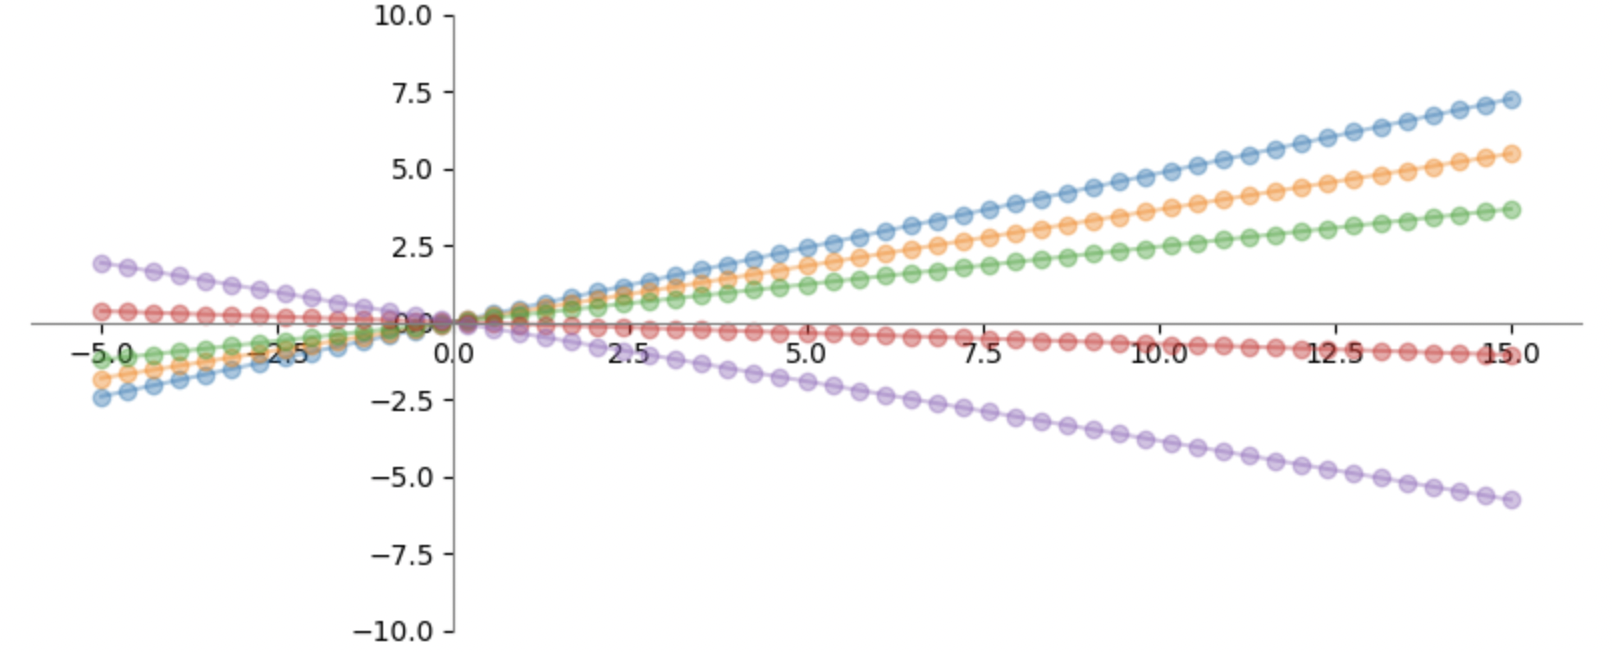
\includegraphics[width=\textwidth]{images/ex3.3.1a.png}
    \end{minipage}
    \begin{minipage}{0.49\textwidth}
        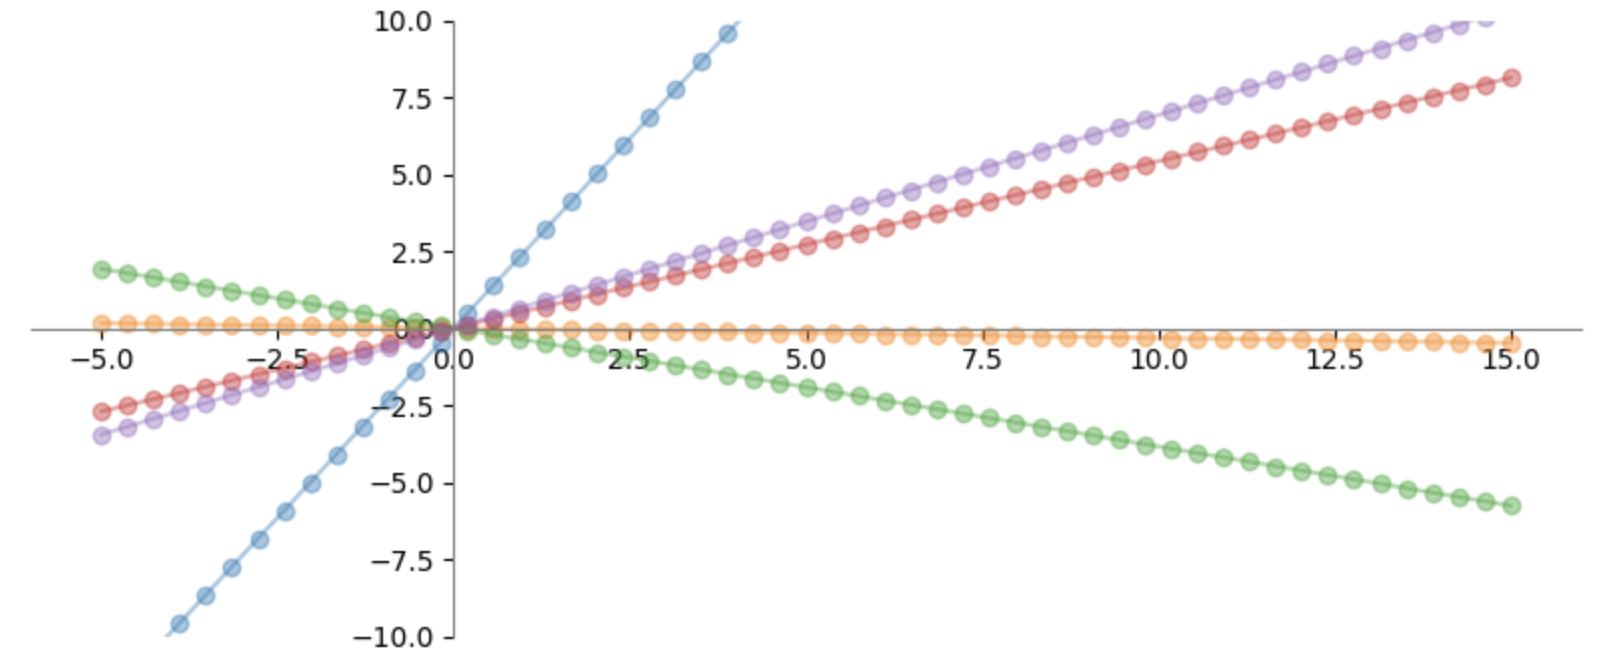
\includegraphics[width=\textwidth]{images/ex3.3.1b.png}
    \end{minipage}

    Keep in mind, that these results are random and will look different each time

\end{frame}

\begin{frame}
    \frametitle{Sampling from a gaussian kernel matrix}

    Sampling 5 vectors twice yields

    \inputminted[bgcolor=LightGray,fontsize=\small]{python}{code/gaussian_sampling.py}

    \begin{minipage}{0.49\textwidth}
        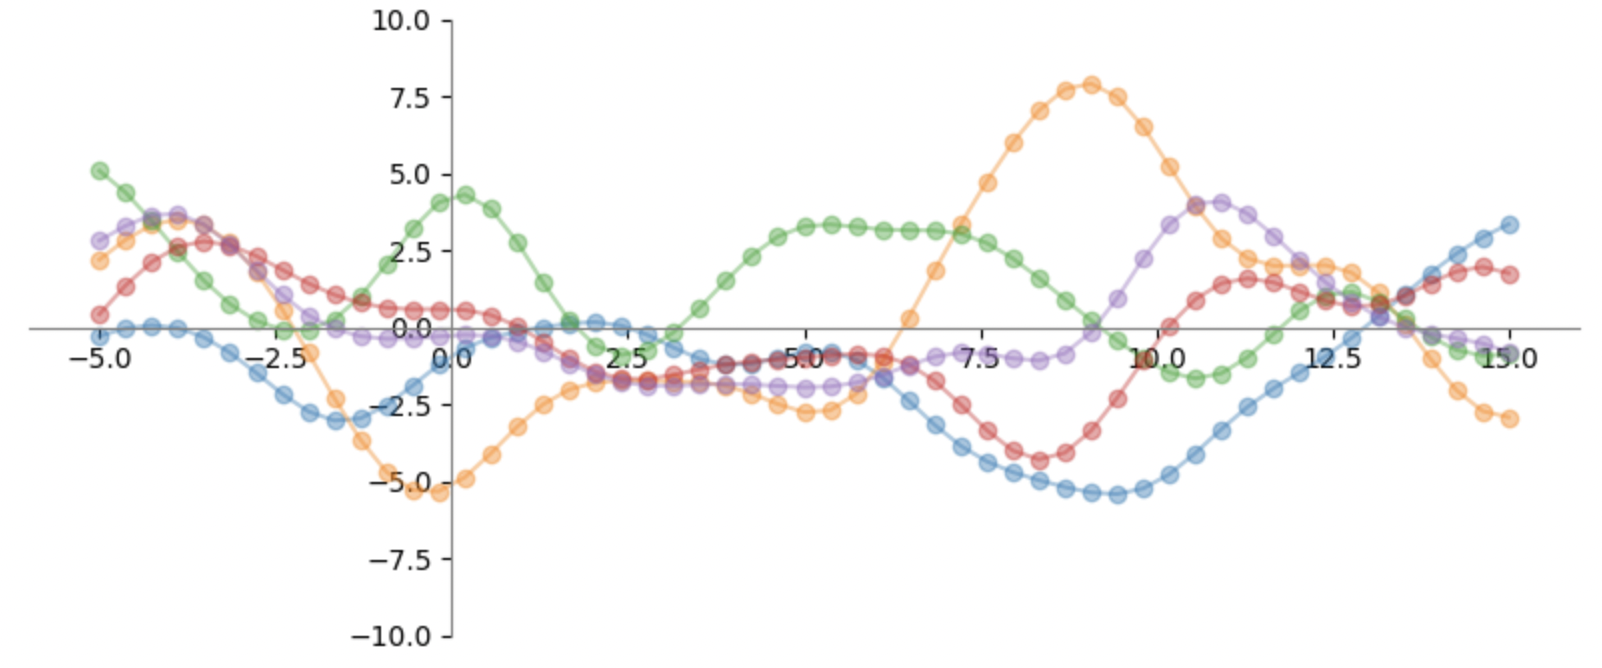
\includegraphics[width=\textwidth]{images/ex3.3.2a.png}
    \end{minipage}
    \begin{minipage}{0.49\textwidth}
        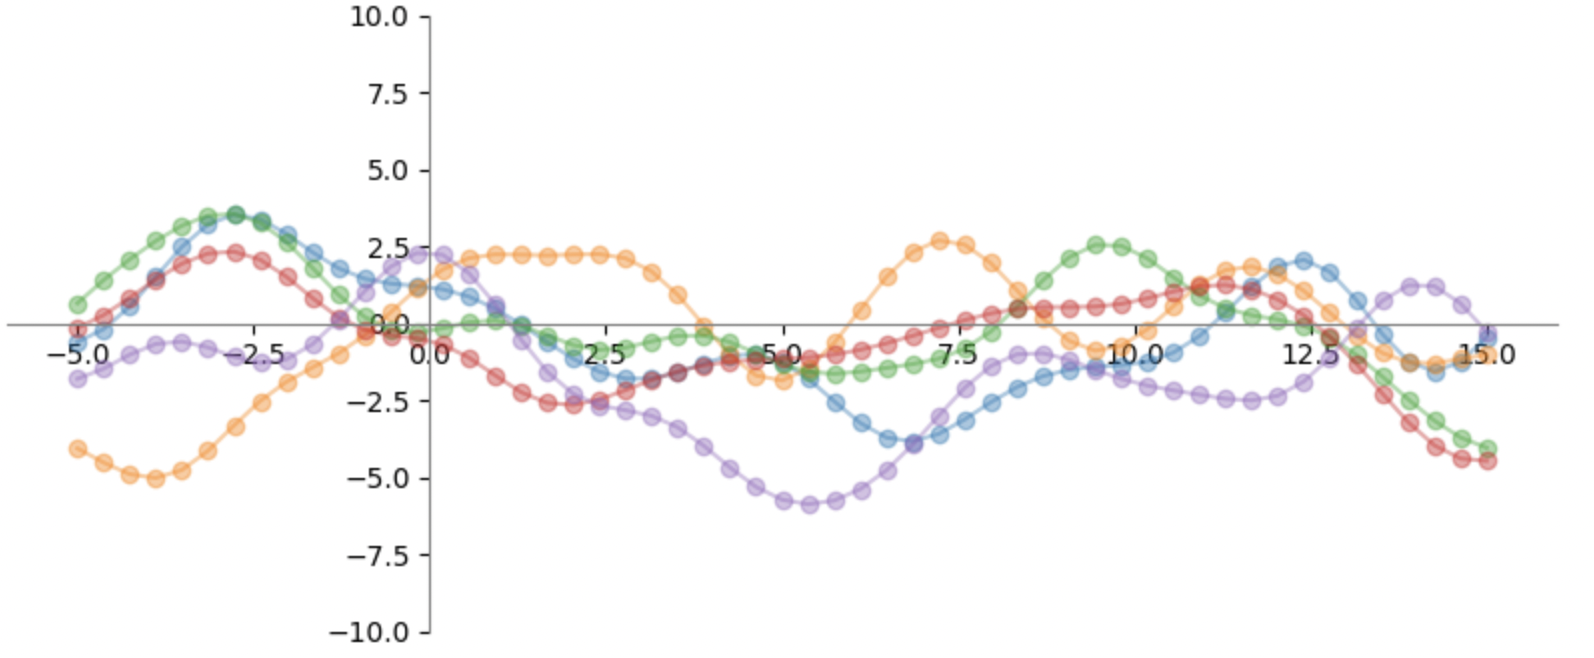
\includegraphics[width=\textwidth]{images/ex3.3.2b.png}
    \end{minipage}

    Keep in mind, that these results are random and will look different each time

\end{frame}

\section{Exercise 3.4}

\begin{frame}
    \frametitle{Fitting a gaussian process to the weight data set}

    \begin{itemize}
        \item Goal: Given the weight and height data from whData.dat, calculate a gaussian process that fits the data
        \item Steps:
            \begin{enumerate}
                \item Remove outliers
                \item Build kernel matrix using  diffMatrix and prodMatrix 
                \begin{align*}
                    [K]_{ij} &= \theta_1\exp\left(-\frac{(x_i-x_j)^2}{2\theta_2^2}\right)+\theta_3 x_ix_j \\
                    C& = K + \theta_4 I
                \end{align*}
                \item Use Scipy.optimize with appropriate bounds to minimize the negative log-likelihood (that is: maximize the log-likelihood)
                using \[\theta=\begin{pmatrix}1.0\\ 20.0\\0.5\\1.0\end{pmatrix}\]
            \end{enumerate}
        \item Result: $\theta=(58.318, 12.507, 0.0, 139.343)^T$
    \end{itemize}

\end{frame}

\begin{frame}
    \frametitle{Fitting a gaussian process to the weight data set}

    \begin{itemize}
        \item Goal: Given the weight and height data from whData.dat, calculate a gaussian process that fits the data
        \item Approach:
            \begin{enumerate}
                \item Remove outliers
                \item Build kernel matrix using  diffMatrix and prodMatrix 
                \begin{align*}
                    [K]_{ij} &= \theta_1\exp\left(-\frac{(x_i-x_j)^2}{2\theta_2^2}\right)+\theta_3 x_ix_j \\
                    C& = K + \theta_4 I
                \end{align*}
                \item Use Scipy.optimize with appropriate bounds to minimize the negative log-likelihood (that is: maximize the log-likelihood)
                using \[\theta=(1.0, 20.0, 0.5, 1.0)^T\]
            \end{enumerate}
            \inputminted[bgcolor=LightGray,fontsize=\small]{python}{code/minimize_nll.py}
        \item Result: $\theta=(58.318, 12.507, 0.0, 139.343)^T$
    \end{itemize}

\end{frame}

\section{Exercise 3.5}

\begin{frame}
    \frametitle{Sampling a fitted Gaussian process model}

    \begin{itemize}
        \item Now that we have a fitted guassian process, we can use our model 
        to sample random pair according to our distribution.
        \item Two mathematically equivalent approaches:
        \begin{enumerate}
            \item Draw $w\sim \overbrace{\mathcal{N}(0,C)}^{=\mathcal{N}(0,K+\theta_4 I)}$
            \item Draw $w\sim \mathcal{N}(0,I)$, calculate a Cholesky factorization $C=LL^T$ and calculate $\overline{y}=Lw$
                \[y'=\underbrace{\overline{y}}_{\text{centered sample}}+\underbrace{\frac{1}{n}11^Ty}_{\text{mean of weights}}\]
        \end{enumerate}
        \item the second approach results in a faster sampling, because it avoids inverting $C$
    \end{itemize}    

\end{frame}

\begin{frame}
    \frametitle{Sampling a fitted Gaussian process model: Results}

    \begin{minipage}{0.49\textwidth}
        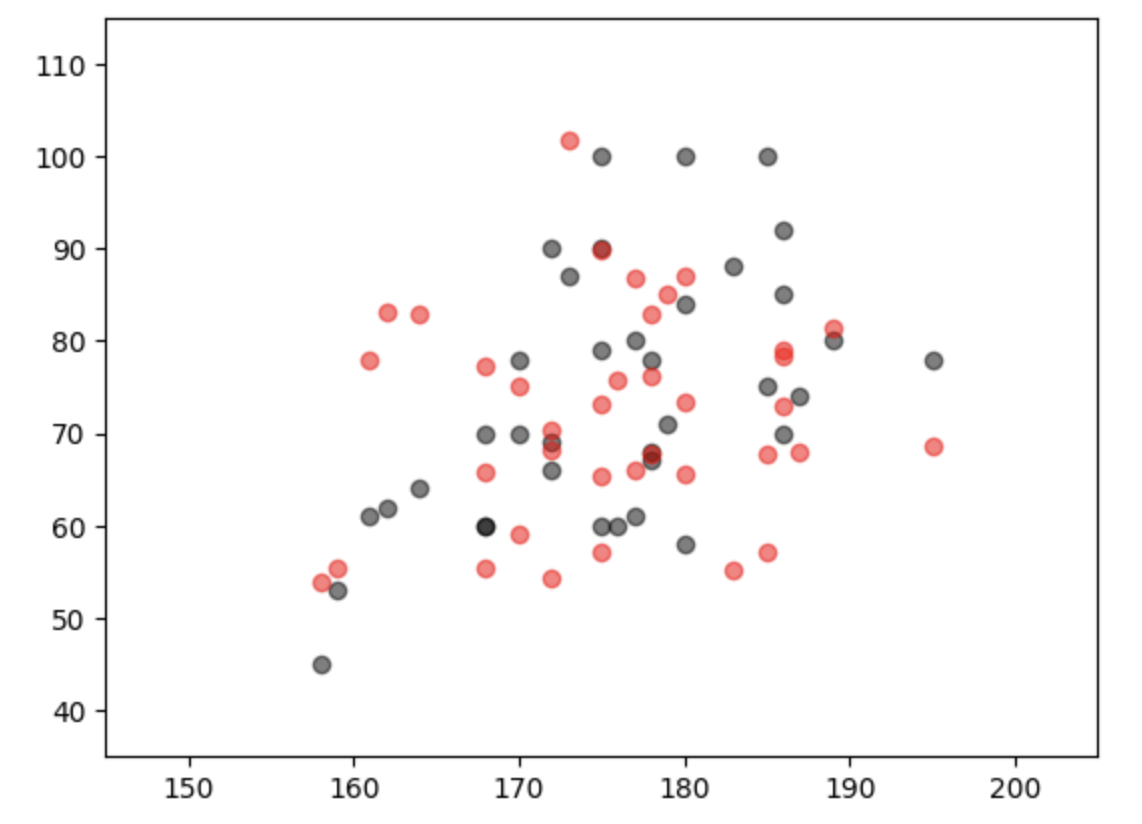
\includegraphics[width=\textwidth]{images/ex3.5.png}
    \end{minipage}
    \begin{minipage}{0.49\textwidth}
        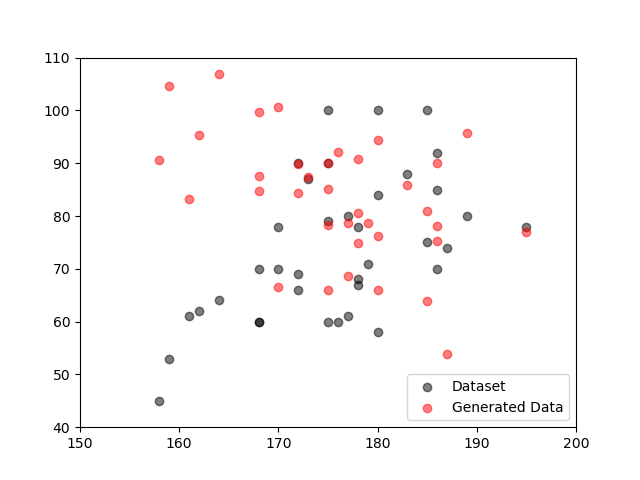
\includegraphics[width=\textwidth]{images/task-3-5-4.png}
    \end{minipage}

\end{frame}

\section{Exercise 3.6}

\begin{frame}
    \frametitle{Predicting with a fitted gaussian model}

    \begin{itemize}
        \item Goal: Predict weights for heights $x^*\in\R^N$
        \item Approach: \begin{enumerate}
            \item Given our fitted gaussian with $\hat{\theta}=(\hat{\theta}_1,\hat{\theta}_2,\hat{\theta}_3,\hat{\theta}_4)^T$
            \item Let
            \begin{align*}
                &K_{xx}=K(x,x,\hat{\theta}_1,\hat{\theta}_2,\hat{\theta}_3)  &K_{x\star}=K(x,x^*,\hat{\theta}_1,\hat{\theta}_2,\hat{\theta}_3), \hspace{3mm}& \dots\\
                &C=K_{xx}+\hat{\theta}_4 I    &\overline{\mu}^\star = K_{\star x}C^{-1}\overline{y},\hspace{9mm}&\Sigma^\star = K_{\star \star}-K_{\star x} C^{-1} K_{x\star}\\
                &\sigma^\star = \sqrt{\text{diag}\left[\Sigma^\star \right]}\hspace{9mm}&\mu^\star = \overline{\mu}^\star +\frac{1}{n}11^Ty
            \end{align*}
        \end{enumerate}
        \item Our predicted height weight pairs are $(x_j^\star,\mu_j^\star)$
        \item We also get a one $\sigma$-confidence $(x_j^\star, \mu_j^\star\pm \sigma_j^\star)$
    \end{itemize}

\end{frame}

\begin{frame}
    \frametitle{Predicting with a fitted gaussian model: Result}

    We get the following plot:

    \begin{minipage}{0.45\textwidth}
        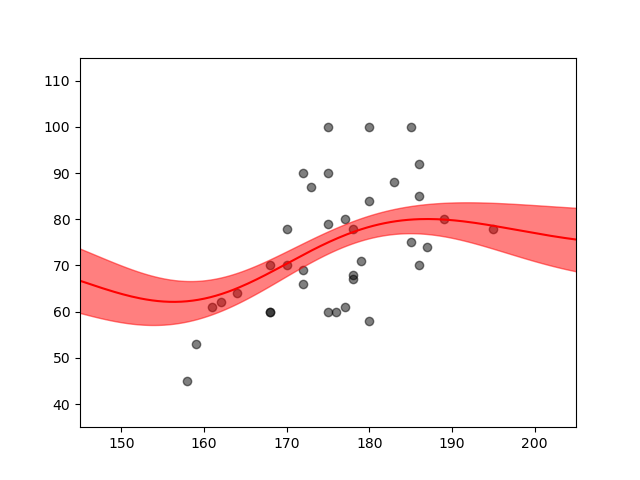
\includegraphics[width=\textwidth]{images/task-3-6.png}
    \end{minipage}
    \begin{minipage}{0.45\textwidth}
        \begin{itemize}
            \item Plot as expected:
            \begin{enumerate}
                \item Thin in the middle (a lot of data)
                \item Greater spread near the lowest / highest weights
            \end{enumerate}
            \item Best model yet, includes with added confidence in each guess.
        \end{itemize}
    \end{minipage}

\end{frame}



\end{document}
